\documentclass[9pt]{beamer}
\usepackage{beamerthemeshadow}
\usepackage{graphicx}
\usepackage{color}
\usepackage[utf8]{inputenc}
\usepackage{hyperref}
\usepackage{setspace}
\usepackage[T1]{fontenc}
\usepackage[flushleft]{threeparttable}
\definecolor{beamer@darkred}{rgb}{0.4,0.15,0.75}
\setbeamercolor{structure}{fg=beamer@darkred}



\def\d{{\fontencoding{T1}\selectfont\dj}}
\def\D{{\fontencoding{T1}\selectfont\DJ}}



\title{Tehničko i naučno pisanje}
\subtitle{Proširena stvarnost i mogćnosti njene primene u obrazovanju}
\author{Matija Đorđević  Filip Nedeljković\\
Mlađan Simić  Igor Stojanović}
\institute{Matematički fakultet\\Univerzitet u Beogradu}
\date{
	\footnotesize{Beograd, 2022.}	
}

\begin{document}

\begin{frame}
	\thispagestyle{empty}
	\titlepage
\end{frame}

\addtocounter{framenumber}{-1}







\begin{frame}
	\frametitle{Pregled} % Table of contents slide, comment this block out to remove it
	\tableofcontents[hidesubsections] 
\end{frame}

\section{Uvod}

\begin{frame}[fragile]\frametitle{Uvod}
	\begin{itemize}	
 \setlength\itemsep{1.5em}
		\item Proširena stvarnost - spoj fizičkog i digitalnog sveta, u kojem digitalni elementi dopunjavaju fizički svet
		\item Razlika između AR i VR - VR zamenjuje predstavljanje stvarnog sveta, dok AR dodaje informacije stvarnom svetu
		\item AR tehnologija nam omogućava da vidimo elemente koji ne postoje u stvarnom životu putem aplikacije kroz ekran uređaja
		\item S obzirom na bogato okruženje za učenje koje nudi AR, istaknuta je i primena ove tehnologije u oblasti obrazovanja.
	
	\end{itemize}
\end{frame}





\section{Istorija}
	\begin{frame}

		
	\end{frame}
\section{Način rada AR tehnologija}
	\begin{frame}

	\end{frame}



 
\section{Primena u obrazovanju}
\subsection{Primena AR  tehnologije u obrazovanju}
	\begin{frame} 
 \frametitle{Primena AR  tehnologije u obrazovanju}
    \begin{itemize}
    \setlength\itemsep{1.5em}
            \item AR i VR se koriste zbog visoke interaktivnosti i sposobnosti predstavljanja virtuelnog okruženja koje podseća na stvarni svet
            \item Istraživanja potvrđuju da tehnološki alati pomažu pri učenju
            \item Moguće je istraživanje i manipulisanje trodimenzionalnim interaktivnim okruženjem 
    \end{itemize}
 
	\end{frame}



 
\subsection{Primeri mogućnosti primene}

 \begin{frame}
 \frametitle{Primeri mogućnosti primene}
            \begin{itemize}
            \setlength\itemsep{1.5em}
		\item Postoje aplikacije koje olakšavaju učenicima da razumeju bolje prostorno okruženje. 
            \end{itemize}
            \begin{figure}[h!]
		\begin{center}
		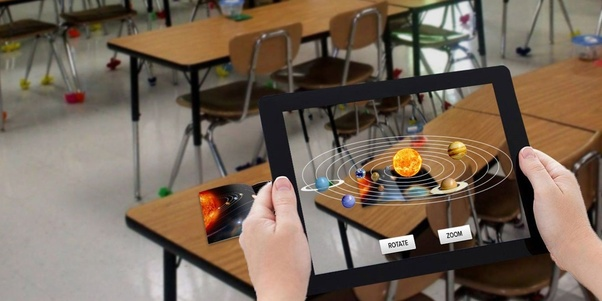
\includegraphics[scale=0.3]{primer.jpg}
		\end{center}
  \begin{itemize}
		\item Proširena stvarnost se može koristiti i kao pomoćno sredstvo u radu sa učenicima koji imaju smetnje u razvoju.
            \end{itemize}
		
		\end{figure}
\end{frame}
